\section{Implementation of RCE-based DAQ for LBNE}


The elements of the DAQ-toolkit described in the previous section can be easily applied to the LAr TPC for LBNE.  The block diagram of a possible configuration is shown in Fig. \ref{fig:blockDiag}.  We define the "front-end DAQ" as everything between the (cold) FPGA and the ATCA shelf; from the ATCA-shelf onward is referred to as the "back-end DAQ".    The primary goal of this document is to propose a solution for the back-end DAQ and so, for this purpose, we will assume that the signals come into the back-end DAQ from the output of the front-end board (FEB) FPGA, each of which collects the output of  $8\times 16 = 128$ TPC wires.  

The basic structure of the back-end RCE-based DAQ is fairly straightforward.  The data from the ADCs is encoded (possibly using the PGP protocol; see Appendix \ref{bll}) in the FEB FPGA and driven out of the cryostat to a "flange board" which converts the electrical signal to an optical signal.  The flange board is an optional step, but one which allows the back-end DAQ crates to be conveniently placed without worrying about signal degradation.   The optical signal is then sent to the RTM which interfaces with the COB.  The RTM also incorporates the output to the DAQ PC farm via 8 x 10 Gbps Ethernet.  The RCEs on the COB can be used to perform event building or even some level of pattern recognition. 

One of the RCEs on each COB will function as the timing interface.  The  external timing  signals will be received via optical fiber to the RTM and will be distributed to the other DPMs and out (through the RTM) to all of the FEBs.  A scheme exists for distributing the timing over the PGP link.  


%Below, we discuss some specific issues with the implementation in the 35t prototype and full LBNE, as well as some ideas for the front-end DAQ.   


%This list is just for me to organize my thoughts.
%\begin{itemize}
%\item \textbf{Data Protocol:  } Implement the PGP protocol over copper from the cold FPGA.
%\item  \textbf{Transition Board:  }  Directly after the cryostat flange (or as part of it)  convert the electrical signals to optical.  This is an optional step, but it allows us to locate the ATCA shelf anywhere without worrying about signal degradation.  Multiple signals into a single board
%\item \textbf{RTM:  } Input is 48 SNAP-12 fiber connectors based on a current (and long utilized) design.  This RTM simply converts optical to electrical and sends the data to the COB  (Is this true???).  Outputs 8 x 10 Gbps ethernet.  
%\item  \textbf{COB:  } Eight independent RCEs with PPC processors used for event building and  pattern recognition or sparsification.  Possibly use RCE FPGA to test sparsification algorithms before implementing them in the cryostat.  
%\item \textbf{ATCA Crate:  }  Provides power and communication between COBs.  Crates available in 2-, 6-, 14-slot varieties. 
%\item \textbf{Triggering:  }
%\item \textbf{Timing:  }
%\end{itemize}



\begin{figure}[hp]
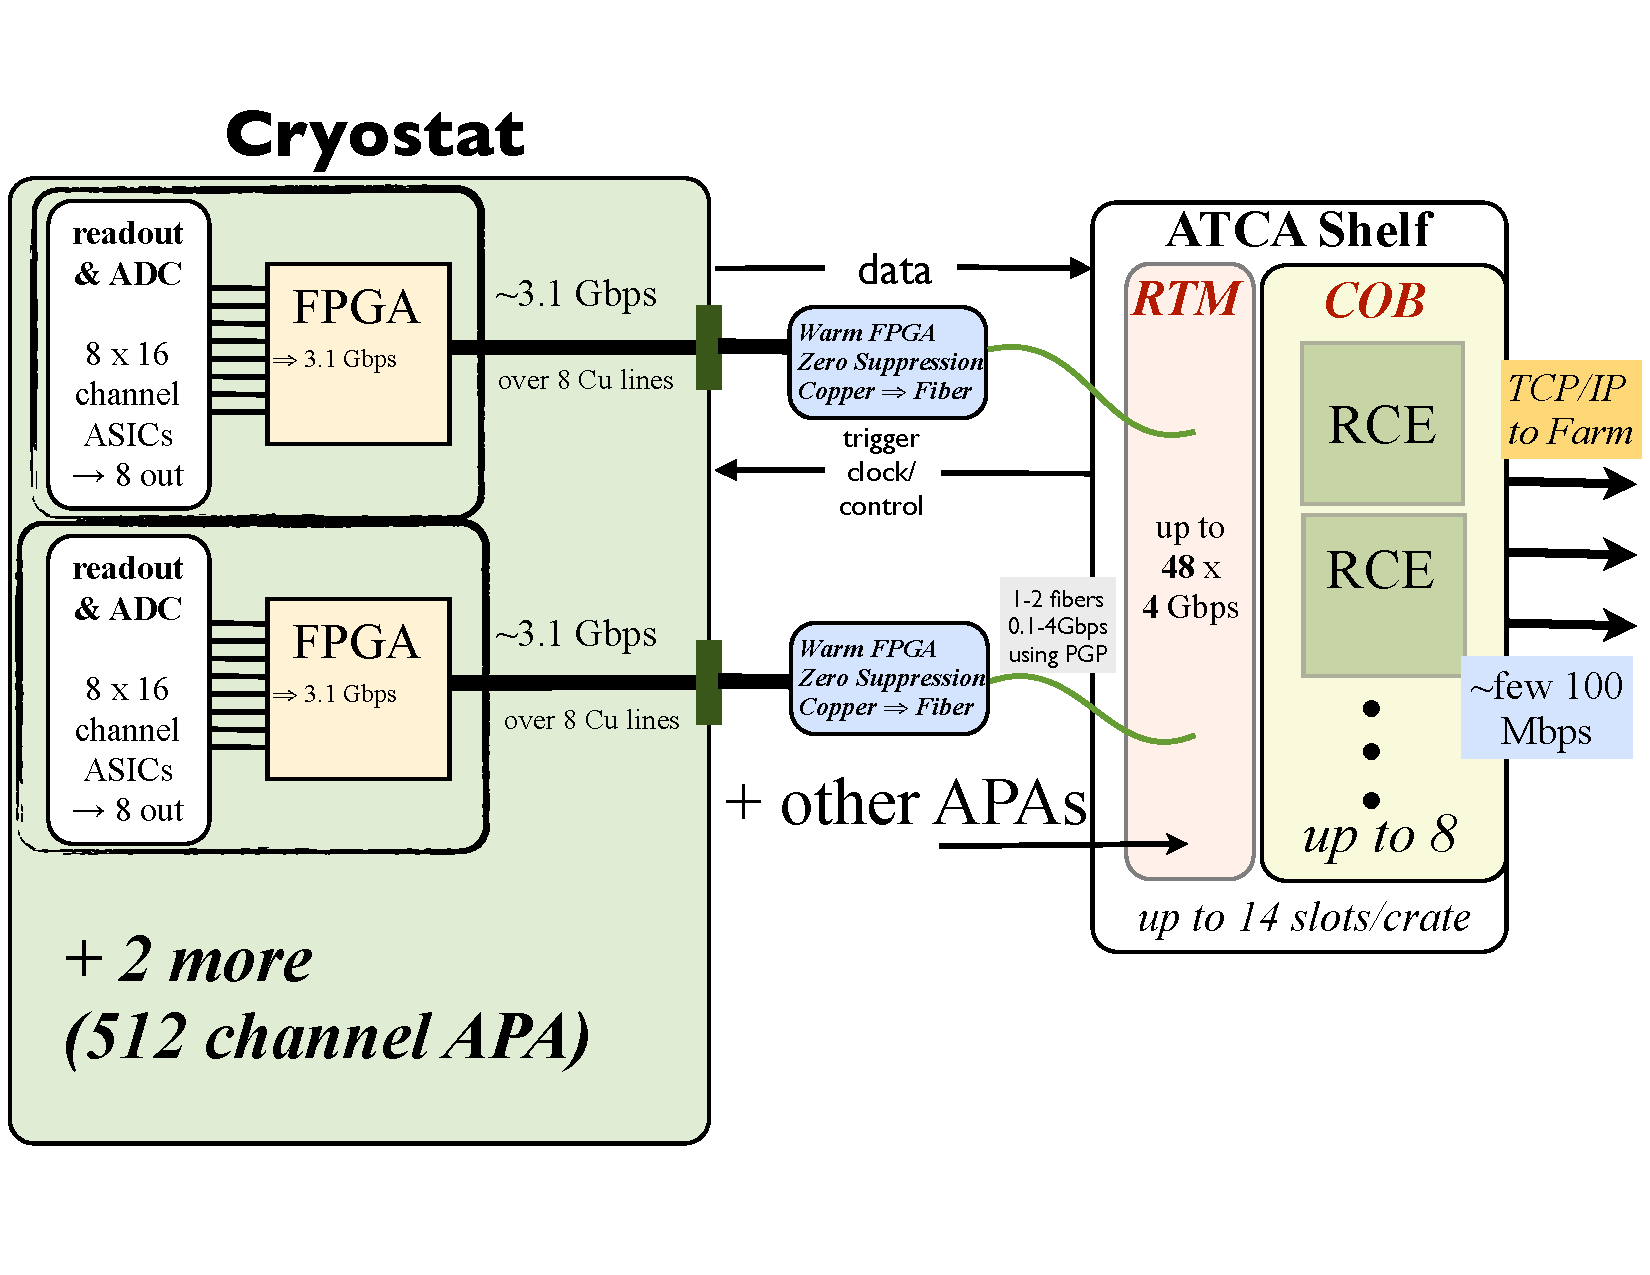
\includegraphics[scale=0.6,angle=90]{LBNE-DAQ-BlockDiagram-35t.pdf}
\caption{Block diagram of the RCE-based DAQ for a single TPC APA in the 35t prototype.}
\label{fig:blockDiag}
\end{figure} 
\clearpage

\subsection{Flange Board}

The electrical signals will be brought out of the cryostat and converted to optical signals just outside the flange on custom built flange boards.   Each flange board houses optical drivers to handle the electrical-optical conversion and to transmit the optical signals to the  back-end DAQ.  The copper side of the flange board will depend on the choices made by the cold electronics group; the fiber side use SNAP-12 transceivers.  The size and number of flange boards depends on the number of connections needed and mechanical specifications.  A block diagram of a two connector board is shown in Fig. \ref{fig:flange}.  Table \ref{tab:daqsumm} assumes four receiver-transmitter pairs per flange board.  

The plan for the 35t prototype is to implement a warm FPGA board that will implement the zero suppression as part of the front end DAQ.  We can implement PGP and place the transceivers on this board and forgo the flange board.  A board with this functionality will be needed for the 10kt, so we've included it as part of the back-end for this proposal.  


\begin{figure}[htb]
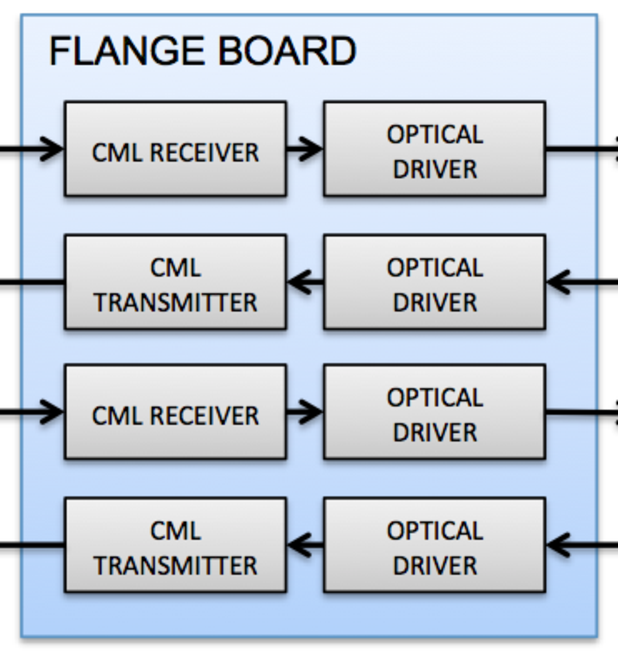
\includegraphics[scale=0.6]{flange-board.pdf}
\caption{Block diagram of a flange board with two pairs of transceivers.}
\label{fig:flange}
\end{figure} 

\subsection{RTM Designs}

RTM designs with up to 48-channel fiber optic inputs (using 4 SNAP-12 transceivers) exist and are currently in use by LCLS and for LSST development. This matches well with LBNE's needs and will require no additional development so our proposal is to use this design.  

The maximum bandwidth/channel into the RTM (and RCEs) is 3.125 Gbps.  For data that is zero-suppressed prior to going into the back-end, this is well above what is needed to read out a FEB.    The bandwidth for full, non-zero suppressed readout of a FEB (which may be advantageous in the prototype) is 3.05 Gbps before accounting for overhead;  this is likely to be $\sim$4 Gbps after 8B/10B conversion and PGP implementation.  Thus, if we prefer to keep the option of reading in all data and performing zero-suppression in the RCEs we'd need to have two data outputs/FEB.   

It is simple (but more time consuming and costly) to design a new RTM and, depending on the final configuration of the front-end electronics, this may be desirable.  For instance, for the photon detector, instead of going through an external digitizer, we could put ADCs directly on the RTM.  This application has been done for the HPS test run and worked well.  


\subsection{COB Configurations}

The COB can be populated with any number between 1 and 8 RCEs, which each RCE servicing 6 input channels.  The RCEs reside on a mezzanine board which can hold up to 2 RCEs/board with up to four mezzanine boards/COB.  The mezzanine boards are "portable"; one may take a mezzanine board out of one COB and put it in another (for instance to expand the channel count of an existing COB).  

For the 35t prototype, assuming 18 channels of TPC data plus at least one other input for timing, we need two fully populated mezzanine boards (4 RCEs).  Alternatively, we could pull 2 outputs/FEB and spread the bandwidth and processing over 36 RTM inputs and 7 RCEs (one for timing). 

%With this configuration, we would have the bandwidth to handle all of the 35t non-zero suppressed data (roughly 4.0Gbps/2 channels, including overhead).  

Each RCE on the COB has a large amount of data processing power (both FPGA and processor based) and the COB itself acts as large bandwidth Ethernet connecting all RCEs.  In addition, each RTM/COB connects to the back-end farm via 8x10Gbps TCP/IP Ethernet links.  This gives us many options for data flow to the back-end CPU farm depending on how much or little data processing we want the DAQ to do.  Some of the options are:
\begin{itemize}
\item use the COB simple as a pass-through; send all data from the front-end to the farm without any modification
\item organize the data into (for example) larger time slices and then send these packets on for further processing and triggering
\item bring the trigger (either beam or cosmic) into the COB and use that to only send out triggered events
\item if reading in non-zero suppressed data, perform zero-suppression (in firmware) and build time slices
\end{itemize}
For this proposal, we do not define a definite role for the RCEs in data processing.  We simply note that using the RCEs can provide some flexibility in designing both the upstream and downstream sides of the data acquisition.  


\subsection{Timing Distribution System}

The timing distribution system for the NOvA detector\cite{Ayres:2007tu} meets the needs of LBNE very well.  The system includes a master timing unit (MTU) with GPS and slave timing units (STU) which can be distributed to the crates about the detector and are self-correcting for propagation delays.  We propose  to use this system as well, both for the full 10kT detector and for the 35t prototype.  For the prototype, this sophisticated system is not strictly necessary; for the RCE-based DAQ there will likely only be one board and the GPS timing isn't required since there is no beam.  However, since there is no hardware (there will be some firmware) to develop and we will need this system for full LBNE we may as include it. 

The NOvA timing system has a fiber optic output which will be used to carry the clock and  be read into one RTM in the crate and then distributed by the COB to all RCEs in the cluster (or possibly 1-per-RTM).  The clock will then be distributed  back through the RTM to the FEBs.   The SFP transceiver on the RTM for the timing signal will be either installed on a RTM daughter board or be included in a custom (though almost trivially different) RTM design.  

\subsection{Photon Detector Readout}


The photon system for the 35t prototype will consist of 32 digitized signals from the output of a CAEN digitizer (some of these may be sync or trigger signals).  From here, there are choices of what to do with the signals.  One option is to simply read them via the USB output into a PC and then forward that data (along with timing information) to the back-end farm, bypassing the RCE-based system entirely.  Alternatively, the digitized signals could be routed to an RTM (possibly in a separate slot) and integrated with the TPC data at that stage.  This option would require some design work for the new RTM.  For this proposal, we've assumed that the photon system bypasses the RCE-based DAQ an goes directly to the farm.  

For full LBNE, we have not included the photon system in this picture as there is not sufficient detail about its layout at this point.   One option, as discussed above, is to include the digitization directly on the RTM.  

%================
\begin{table}[tbh]
\begin{center}
\begin{tabular}{|l|c|c|}   
\hline \hline 
    & 35t  & 10kt \\      
\hline
   Total Channels        & $\sim$2.3k &$\sim$307k \\ 
	Number of APAs     &  3     &    120        \\ 
   Number of FEBs       & 18 & 2400 \\ 
   Flange Boards    & 0   & 50 \\ 
   RTM+COB Boards    & 1  &  50  \\
  RCEs                       & 3  &  400  \\
   ATCA Crates            & 1   &  4 (14-slot)   \\ 
\hline \hline
\end{tabular}
\caption[]{DAQ-related quantities for the 35t and full LBNE (as of Jan. 2013 design).  The assumption is that we will readout one wire/FEB.}
\label{tab:daqsumm} 
\end{center}
\end{table}
%=================



\subsection{Summary DAQ Layout for 35t Prototype and Full LBNE}

The number of boards/RCEs/crates etc needed for the 35t prototype and 10kt LBNE is listed in Table \ref{tab:daqsumm}.  

35t Phase-II:  
\begin{itemize}
\item  \textbf{TPC RTM: }  4 pairs of SNAP-12 transceivers + SFP (timing)
\item  \textbf{TPC COB:  }  2 mezzanine boards each with 2 RCEs (4/8 for full readout)
\item  \textbf{Timing Distribution:  }    Single NOvA MTU/STU pair
 \item  \textbf{Photon Detector:  }    digitizer to PC to back-end farm 
\end{itemize}


Full LBNE:
\begin{itemize}
\item  \textbf{TPC RTM: }  4 pairs of SNAP-12 transceivers 
\item  \textbf{TPC COB:  }  4 mezzanine boards each with 8 RCEs (i.e. fully populated)
\item  \textbf{Timing Distribution:  }    Single NOvA MTU + 4 STU (one for each crate)
 \item  \textbf{Photon Detector:  }    analog signals to RTM, which contains ADC
\end{itemize}
%The 35t prototype TPC will have $\sim 100\times$ fewer channels than the full LBNE TPC and additionally will be externally triggered to observe cosmic rays.  The trigger rate is estimated to be  $<1$kHz.  If we run out a single wire/FEB from the cryostat, then the entire TPC can be read into a single COB.  
%Bringing more wires/FEB would require more COBs; the maximum number of input channels/RTM is 48.  For 8 wires/FEB, 4 COBs are likely required, since the trigger and timing signals will take up one input to the RTM each.  

%In total, even if multiple wires/FEB are read out, the 35t DAQ will easily fit into a single ATCA shelf. 

%================
%\begin{table}[tbh]
%\begin{center}
%\begin{tabular}{|l|c|c|c|}   
%\hline \hline 
 %   											&    per-FEB               &       35t   Total   & Full LBNE  Total \\      
%\hline
%   Full Readout 2MHz  			  & 3.05 Gbps & 54.9 Gbps  &  7320 Gbps \\ 
 %  Zero-suppressed cosmics  & 15~-~?? Mbps& 270~-~?? Mbps  &  36~-~??  Gbps\\ 
  %Radioactivity  ($^{39}$Ar)    & 0.6 Mbps&  11 Mbps  &   1.4 Gbps \\
 %  Electronics noise& 0.01 Mbps & 0.18 Mbps&  24 Mbps\\ 
%\hline \hline
%\end{tabular}
%\caption[]{Estimated data rates per 128-channel FEB and for the entire 35t and full LBNE TPCs  (mostly from J. Urheim).}
%\label{tab:datarates} 
%\end{center}
%\end{table}
%=================

%\subsection{Summary of DAQ Layout for 10kT LBNE}


\subsection{Comparison of RCE-based vs DCM-based back-end DAQ Systems}

The baseline design for the LBNE DAQ \cite{DAQ_CD1}
is based on Data Concentrator Modules (DCMs) 
that were originally designed for use in the Nova experiment.
Each of these modules takes 64 input data data streams of 20 Mbps and 
combine them into a single stream of 1 Gbps. 
The total throughput of a DCM module is limited to 60 Mbytes/second.
A single DCM module is thus able to handle enough data to readout the
entire 35 ton prototype at the expected rate of 300 Mbit/second/APA,
although without a large amount of headroom.
The main advantage of an RCE-based system is a vast improvement
in the available bandwidth, which adds signficant flexibility in 
the handling of the raw datastream.
For example, much high noise rates could be handled.
As an extreme example, one could consider reading non-zero-suppressed data 
into the DAQ system.




%\subsection{High-speed Data Links From Cold FPGA to back-end DAQ}

%...possibilities and our plans on this ...

